%!TEX root = ../BoYu-Dissertation.tex
\graphicspath{{Figures/}}

\chapter{Our Approach: Knowledge Updating} % (fold)
\label{cha:knowledge_updating}
The knowledge updating in this chapter covers two important issues: on one hand is updating the knowledge representation of the field of work so that it always reflects the current state of the collaborative activity by reacting to the various external and internal events through several reasoning processes. On the other hand, these reasoning processes also enrich these events with system generated knowledge that is used to support the human actor's awareness processes in following chapters. In the following, we first provide an overview of the knowledge updating process, and then describe each component in detail.

\section{Knowledge updating process} % (fold)
\label{sec:knowledge_updating_process}
Each time when the system detects that there is a new event, it triggers the knowledge updating process to decide how it influences the state of the field of work and update the correspondent in the PlanGraph. In general, the knowledge updating is a four-step process of \emph{association}, \emph{assessment}, \emph{elaboration}, and \emph{propagation}.
\begin{enumerate}
	\item \emph{Association}. The knowledge updating starts with the association of an event with the field of work. In this step, the system searches the current PlanGraph model for an appropriate match between the input event and the entities or relations in the field of work. If a match is found, the system uses the information stored in the event to update the PlanGraph.
	\item \emph{Assessment}. The second step is to assess how the event can contribute to new changes in the collaborative activity. It may trigger new actions that need to be added to the field of work, or change the current state of existing actions. 
	\item \emph{Elaboration}. Based on the assessment of new changes, the elaboration step is to reason about the system's expectation on any new actions that need to be added to the field of work, or what actors will be potentially involved in these new actions. This is usually performed with domain specific knowledge, such as recipes of performing an action, and the specification of role responsibility.
	\item \emph{Propagation}. The propagation step focuses on evaluating how the current change can be possibly propagated other actions in the field of work because of the dependencies among them. 
\end{enumerate}

The four steps of knowledge updating process share some commonality with the human actor's awareness development processes. The \emph{association} and \emph{assessment} steps are very similar to the \emph{comprehension} process, where the actor comprehend or understand the relevance of awareness information in relation to its tasks and goals. The \emph{elaboration} and \emph{propagation} can be considered as the projection of the states in the near future, as the actor forecasts likely future states in the situation. In this way, we can think of the knowledge updating process as the computer system's awareness development process. The only difference is that, as the human actor usually only needs to be aware of things in his/her local scope of work, the computer system aims to possesses the knowledge of the whole field of work through the knowledge updating.

One thing to note is that not every event will be processed through all the four steps. Some external event may not directly link to any entity in the field of work, or the system does not have the complete knowledge to assess its implication on the field of work. In such case, the event will be passed by to the human actors for interpretation. The result of human actor's interpretation as a new internal event then starts a new round of knowledge updating, during which the system's knowledge is updated.

As we emphasize in the beginning, the knowledge updating is a two-way process, i.e. while the PlanGraph model of the field of work is updated by the new event, the event itself is also developed in the system's reasoning processes. For example, in the \emph{assessment} step, an external event \emph{`TrafficBlocked'} causes the system to believe that the action to delivery a resource to an actor cannot be achieved, i.e. a new internal event describing the system's belief about the state change on the delivery action can be derived. Later, in the \emph{propagation} step, the system may generate a new internal event to indicate that because of the state change on the delivery action, the actor's action that is waiting for the resource delivery will also be impacted. In this way, the original event is derived into a chain of events as the knowledge updating process proceeds.

To recording the development of an event in the knowledge updating process, we define an \emph{event chain} $\Theta$ as an ordered sequence of events: $\Theta=(e_0, e_1, e_2, ...)$. In the beginning of the knowledge updating process, there may be only one event $e_0$, i.e the original external event in the event chain $\Theta$. As the knowledge updating proceeds, more events are added to the chain. In the assessment step, the system may generate derived events indicating the system's belief on how the field of work has been changed due to the original events. In the propagation step, the system predicates the future state changes, and attaches more anticipatory events to the chain. Figure \ref{fig:knowledge_updating} shows the knowledge updating process with the development of the event chain.
\begin{figure}[htbp] %  figure placement: here, top, bottom, or page
	\centering
	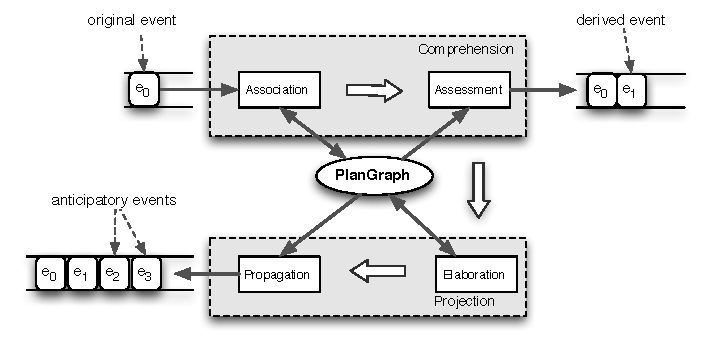
\includegraphics{knowledge_updating.pdf} 
	\caption{The knowledge updating process}
	\label{fig:knowledge_updating}
\end{figure}
% section knowledge_updating_process (end)

\section{Step 1: Association} % (fold)
\label{sec:step_1_association}
The knowledge updating starts with establishing the association between the input event and the current PlanGraph model representing the field of work, and use the event information to update the PlanGraph model. The association starts with the recognition of event type for each input event, as the different event types are treated differently.

If the event is an \emph{external event} on entities, we consider the following two cases:
\begin{enumerate}
	\item If the event is indicating an existential change over time, the event is directly passed through to the assessment step, as the entity linked to this event did not exist in the past.
	\item Otherwise, we search all the PlanGraph nodes to find any match with the entity described in the event based on their unique identifiers. If a match is found, we update the attribute information attached with the PlanGraph node based on the event type. If it is a state change event, we change the state of th node. If it is an existential change over space, we update the location information of the node. If it is a value comparison event, we update the corresponding attribute value. After updating the node, we add an entity reference in the event object, so that it can direct link to the matched PlanGraph node for later use.
\end{enumerate}

If the event is an \emph{external event} on relations, we check for the following cases:
\begin{enumerate}
	\item If the event indicates a resource assignment relation, i.e. a resource $res_1$ is assigned to the performance of an action $act_1$. we search all the action nodes in the PlanGraph to find any match with the action entity described in the event $act_1$. If a match is found, we search for the parameters of $act_1$ in the PlanGraph to find any of them has the same resource type as $res_1$ and then assign the values of $res_1$ to the parameter. After that, we add an entity reference pointing to the parameter node in the event's payload. 
	\item If the event indicating a structural relation, e.g. an action $act_2$ is a subsidiary action of another action $act_1$. we search all the action nodes in the PlanGraph to find any match with the action entity $act_1$ described in the event. If a match is found, we create a new node with the information described in $act_2$, and then add an entity reference pointing to this new node into the event's payload. This can be applied to other decomposition relations, such as an action is a subsidiary action to achieve a condition, or a new parameter needs to be added to an existing action.
\end{enumerate}

If the event is an \emph{internal event}, we consider the following cases:
\begin{enumerate}
	\item If the event is an \emph{intention event}, we search all the action nodes in the PlanGraph to find any match with the action entity described in the event. If a match is found, we search for the \emph{Intentions} associated with the action node to find any existing actor has the same identifier as the actor entity described in the event. If so, we update the intention type based on the intention event. Otherwise, we add the actor and the corresponding intention into the the \emph{Intentions} associated with the action node. After that, we add an entity reference pointing to the action node in the event's payload. 
	\item If the event is a \emph{belief event} about an actor's capability to perform an action, we search all the action nodes in the PlanGraph to find any match with the action entity described in the event. If a match is found, we search for the \emph{Capabilities} associated with the action node to find any existing actor has the same identifier as the actor entity described in the event. If so, we update the capability type based on the belief event. Otherwise, we add the actor and the corresponding intention into the the \emph{Capabilities} associated with the action node. After that, we add an entity reference pointing to the action node in the event's payload. 
	\item If the event is other \emph{belief events}, we apply the association rules directly on the subsidiary event describing the content of the belief. 
\end{enumerate}

In sum, two results are achieved if an association between the event and the PlanGraph model is found in this step. First, the corresponding PlanGraph entity or relation is updated based on the new information carried by the event. Second, the event is enriched with a direct link to the corresponding PlanGraph node, that is the context of origin of this event is identified. 

However, not all the events are directly associated with the PlanGraph model. As we discussed in Section \ref{ssub:external_events}, some external events may describe occurrence on the entities that are not currently in the PlanGraph, but implicitly impact the field of work by motivating new actions or implying the effects of action performance. These events will be passed through to the assessment step for further analysis. 
% section association (end)

\section{Step 2: Assessment} % (fold)
\label{sec:assessment}
In the assessment step, each event is evaluated to check how it can lead to changes towards the action performance, such as the execution state change of an action, or a condition. The changes towards action performance can be explicitly expressed in the event, and is directly associated with the action node during the association step. For example, it can be an internal event from a human actor indicating the belief that the resource delivery action has been successfully performed. However, in the assessment step, the system is more interested in the events that impact the action performance implicitly, where inference becomes necessary. For example, an external event indicating that a resource is now located at an actor's position can implicitly indicate the successful performance of the resource delivery action. In this case, a new event showing the state change of the resource delivery action will be derived and added to the event chain along with the original event.

The knowledge stored in the PlanGraph allows the system to perform some routine assessment tasks that are universal across different application domains. Some of the basic inference tasks can be described as follow:
\begin{enumerate}
	\item \emph{Goal conditions on action nodes}. If an event describes changes on entities or relations that are included in an action's goal condition, the system can evaluate the action's goal condition. If the goal condition becomes holding because of this event, we derive a new state change event on this action, and push it into the event chain.
	\item \emph{Condition nodes}. If an event describes changes on entities or relations that are included in a condition node, the system can evaluate the condition node. If the condition becomes holding or no longer holding because of this event, we derive a new state change event on this condition, and push it into the event chain. 
	\item \emph{Parameter nodes}. If an event describes changes on an resource that is assigned to a parameter node, the system can evaluate the parameter's subsidiary conditions. If a  condition becomes holding or no longer holding because of this event because of this event, we derive a new state change event on this parameter, and push it into the event chain.
\end{enumerate}

The second type of tasks that the system can perform during the assessment process is to check whether the event can activate new action that needs to be added to the field of work. This type of events is usually called \emph{triggering events}, as they are often not directly associated with any current nodes in the PlanGraph, but will trigger some new action to be performed. For example, every time a new victim is found in an emergency response operation will trigger a new rescue action to be performed. In this case, the initial event about the discovery of a new victim cannot be associated with any existing actions, but asks for a new action to be performed. The assessment of action activation requires a set of pre-defined domain-specific activation rules, so that every event can be searched through the activation rules to find whether it satisfies any of the conditions. If so, a new action is added to the field of work as a new PlanGraph, and the new derived event is generated to indicate the activation of the new action.

Furthermore, the assessment step can involve more sophisticated inference techniques, such as spatio-temporal reasoning \cite{Bennett}, pattern recognition \cite{zelnik2001event}, or case-based reasoning \cite{jakobson2004towards}, to enhance the system's reasoning capabilities. However, these reasoning techniques often require a great number of domain knowledge, and lack flexibility to handle unexpected events. As we discussed in Section \ref{sub:human_computer_collaboration}, one of the design principles of our approach is to leverage the different capabilities of computers and humans. As a result, in the assessment step, we design the system to focus on the more reliable low-level routine inferences that can be directly performed in the PlanGraph model, and leave the complex, higher level assessment to the human actors. Hence,
some events may not be considered as contributing to the collaborative activity by the system in the assessment process. Rather, they are later interpreted by human actors and send back to the system as internal events, which will then be used to update the system knowledge.
% section assessment (end)

\section{Step 3: Elaboration} % (fold)
\label{sec:step_3_elaboration}
The main goal in elaboration step is to advance the collaborative activity from the system side based on the change from the new event. After the assessment process, the context of the activity is changed, and the system attempts to elaborate the PlanGraph to accommodate the changes. 

Based on the specification of SharedPlan theory \cite{Grosz2006}, the system can elaborate the current PlanGraph in several ways. 
\begin{enumerate}
	\item \emph{Recipe selection}. The system can contribute to the collaborative activity by retrieving a recipe for a new action from the knowledge base, i.e. by providing a default way to perform this new action.
	\item \emph{Parameter binding}. If any of the parameters is unbound to any values, the system will search the knowledge base to find any action that can be performed to identify the value for the parameter.
	\item \emph{Condition satisfaction}. If any of the pre-conditions is not holding, the system will search the knowledge base to find any action that can be performed to satisfy the condition.
	\item \emph{Actor allocation}. If any of the actions has not been committed by any actors, the system search for the actors who might be potentially intended to or capable of performing the action. 
\end{enumerate}

The elaboration step is not performed for every event, rather it is only triggered by a subset of events that are related to the development of the collaborative activity. 
\begin{enumerate}
	\item Events on structural relations. Whenever an event indicates that a new action is a subsidiary action to another action, a way to identify a parameter, or to achieve a condition, the new action will be added to the PlanGraph in the association step, and needs to be elaborated.
	\item Events on goal activation. The elaboration needs to be performed whenever a new action has been added to the field of work because of some triggering event during the assessment step.
	\item Events leading to condition violation. Whenever an event leads to the fact that some condition is no longer holding in the assessment step, the elaboration needs to be performed on the condition node to identify any action that can be performed to satisfy it.
\end{enumerate}

The elaboration process is achieved with the support of two types of pre-defined knowledge: (1) the recipe knowledge about how to derive an action into a sequence of parameters, pre-conditions, and subsidiary actions, how to identify a unbound parameter, or how to satisfy a condition, etc.; (2) the knowledge about actor roles and their corresponding responsibilities and capabilities. The former allows the system to extend the field of work by adding new action, parameter, or condition nodes into the PlanGraph model, and the knowledge about actor roles allow the system to reason about who are likely to be interested in these newly added entities, or who have the capability to work on these new entities, so that the system can extend the actors' local scopes to these newly added entities.

The elaboration process is predictive as it reflects the system's prediction on how the collaborative activity will be advanced based on the new event occurrence. The system provides a default plan of performing an action, and identifies the potential actors who might be interested in it. After the elaboration process, the PlanGraph not only reflects the current state of the collaborative activity, but also shows the potential next steps based on the system's knowledge. However, the results of elaboration process never dictate how the human actors will eventually develop the action. The human actors may later generate new internal events to revise the plan generated by the system, or change their intention/capability levels towards the action in the PlanGraph.
% section step_3_elaboration (end)

\section{Step 4: Propagation} % (fold)
\label{sec:step_4_propagation}
Propagation is another predictive process that the system can perform to predict future state changes in the field of work. It is triggered by the events that either directly indicate (in the association step) or imply (in the assessment step) state changes on the entities in the filed of work, and then reason about how these initial state changes can be propagated to other actions due to the multiple dependencies between them. A simple example could be be: if the execution state of an action $act_1$ is changed from \emph{executing} to \emph{failed}, then the parent action $act_2$ (i.e. $SubAct(act_1, act_2)$ holds) will likely to be impacted and may be also changed to \emph{failed} if the plan is not changed. 

The propagation is performed on the dependency network, which can be easily constructed from the PlanGraph model (Section \ref{sub:representing_dependencies}). The dependency network abstracts away the detailed information on each action node and focuses on the dependency relationships among them, we can adopt more efficient network-based reasoning models to perform the propagation. In this study, we employ the Bayesian network to perform the propagation \cite{pearl1988probabilistic}. Bayesian networks are directed acyclic graphs in which the nodes represent multi-valued variables, and the arcs signify direct dependencies between the linked variables and the strength of these dependencies are quantified by conditional probabilities. The purpose of the Bayesian network is to give a belief in each possible value for each node after some evidence arrives.

In the context of our model, the nodes are the basic elements in a dependency network, i.e. dependers, dependums, and dependees, which represent the entities in the field of work, i.e.  actions, resources, or conditions. The evidence fed into the network includes certain state changes on these entities. Thus, the purpose of the Bayesian network is to update the system’s belief in the states for every other node after some state change occurs on a node.

To operationalize the Bayesian network, we need to follow the following steps: (1) construct the Bayesian network, (2) assign the conditional probabilities for each link, (3) and perform the belief updating when some events arrive.

\paragraph*{Construction of Bayesian networks} % (fold)
\label{par:construction_of_bayesian_networks}
By following the algorithm in Section \ref{sub:representing_dependencies}, we can construct the dependency network from the PlanGraph model, and then the construction of Bayesian network is very straightforward. We translate each basic element in the dependency network into a node variable, and the different dependency relationships into corresponding links in the Bayesian network. The possible values for each node are determined based on the possible execution states for each type of node variables. At a given time, an action can be at one of the following states: \emph{inactive}, \emph{planning}, \emph{executing}, \emph{complete}, \emph{failing}, and \emph{delaying}. Each condition can be \emph{open}, \emph{waiting}, or \emph{holding}. Each resource can be \emph{unavailable}, \emph{waiting}, or \emph{available}. Figure \ref{fig:state_transitions} shows all the states for each type of node and the possible state transitions.
\begin{figure}[htbp] %  figure placement: here, top, bottom, or page
	\centering
	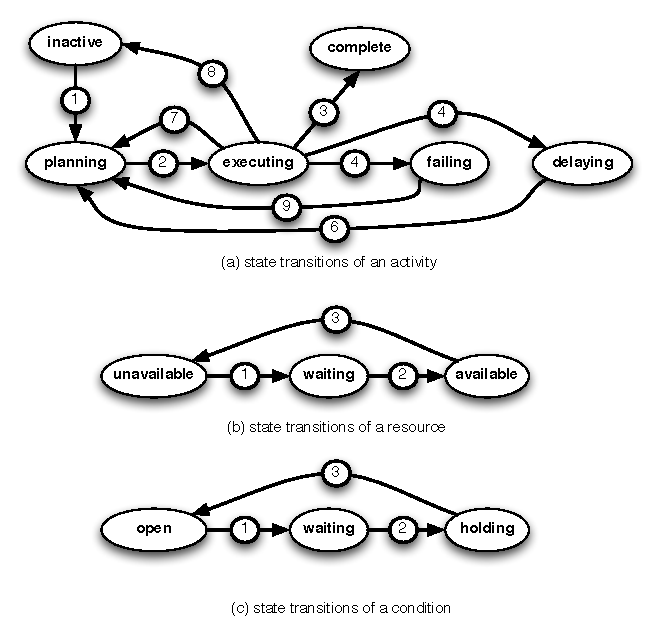
\includegraphics{state_transitions.pdf} 
	\caption{Types of node variables and their possible values in a Bayesian network}
	\label{fig:state_transitions}
\end{figure}
% paragraph construction_of_bayesian_networks (end)
\paragraph*{Assignment of conditional probabilities} % (fold)
\label{par:assignment_of_conditional_probabilities}
Before any propagation commences, we need to assign the conditional probabilities for each node that form the conditional probability matrices. An element of the conditional probability matrix looks like $P(x_i|u_{1j_1}, ..., u_{nj_n})$, and gives the probability of state $i$ for node $x$ conditioned on the states of its parent nodes. For example, the conditional probability of an action node indicates the possibility of each state for this action, given the states of all the resources, conditions, actions that it depends on. 

\fxwarning{showing an example of the conditional probability table}
\fxwarning{add an appendix showing the algorithm for the assignment}

In our study, we develop a set of heuristic rules to assign the initial conditional probabilities for each type of nodes, by evaluating the criticality of each parent node, and the opportunities for re-planning. For example, if a critical resource is needed for every possible way to perform an action, the state of the resource as \emph{failing} will definitely lead to the \emph{failing} of the action. However, if there are other possible plans to perform the action that do not require this resource, the probability of the action being failing will be decreased.

The assignment of conditional probabilities provides the system with the default reasoning capability to propagate the state changes that can be later overwritten by the user's interpretation. When a user changes the belief in the state of an activity, the change will overwrite the system’s initial belief through the belief updating. Because of this interactive nature, the purpose of the initial probability assignment is just to provide a good guess about the propagation from the system's perspective and does not have to be perfectly accurate. 
% paragraph assignment_of_conditional_probabilities (end)

\paragraph*{Belief Updating} % (fold)
\label{par:belief_updating}
We follow Pearl’s belief propagation algorithm \cite{pearl1988probabilistic} to perform belief updating whenever a state change occurs. In this approach, the belief in each value of a node variable is divided into two parts: the part emerges from its ancestors and the part emerges from its descendants, and the final belief is ascribed by multiplying the two parts. As a result, the belief updating is performed as a bidirectional propagation process. 
\begin{enumerate}
	\item Starting at the node where the initial state change occurs, the system calculates how the state change will change the beliefs on each parent node. If the change on a parent node is significant, i.e. above a given threshold, the parent node becomes active, and will be further propagated to its parent. This is called \emph{causal} propagation since the updating is from a cause to an effect to indicate how a state change of the cause will lead to the change of the effect. 
	\item On the other hand, the belief updating can also calculated from an active node to their children. This is called \emph{evidential} propagation as the reasoning flows from evidence to hypothesis.
\end{enumerate}

In our approach, both the causal and evidential propagation will be performed. The causal propagation is used to provide the system's predicted state changes on the actions that are dependent on the action where initial state change occurs. The evidential propagation occurs whenever a user modifies the system’s prediction on a given node and the system uses it as an evidence to trace back and revise the previous beliefs on the dependees.
% paragraph belief_updating (end)

The result of the Bayesian network-based propagation will be used to enrich the event chain with anticipatory events. Starting from the node that the initial event is linked to, the system use the previous probability distribution before the propagation and the current values to perform the Cartesian product on each node. Each value in the new two-dimension table indicates the probability of each possible state change. If a significant state change has been detected (by comparing with pre-defined threshold), it will be added to the event chain as a new anticipatory event. For example, Figure \ref{fig:prob_state_change} shows the result of a propagation process on a parameter node. Before the propagation, the parameter had a high probability to be in the state of \emph{waiting}, and after the propagation, the probability distribution changed. By calculating the Cartesian product, we can find the most significant state change on the node is from \emph{waiting} to \emph{delay}, with a confidence level of $0.83808$. As a result, a new anticipatory event indicating that the state of this parameter has been changed from \emph{waiting} to \emph{delay} will be pushed into the event chain.
\begin{figure}[htbp] %  figure placement: here, top, bottom, or page
	\centering
	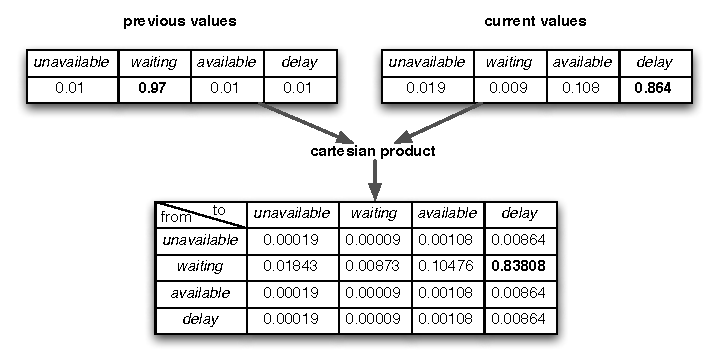
\includegraphics{prob_state_change.pdf} 
	\caption{An example of calculating state-change probabilities}
	\label{fig:prob_state_change}
\end{figure}
% section step_4_propagation (end)
\section{An Example} % (fold)
\label{sec:an_example}
To demonstrate the knowledge updating process, we consider a simplified version of the victim rescue activity in the emergency response scenario to see how the PlanGraph model of the field of work is updated through several consecutive events, and meanwhile the events are enriched into event chains. The task involved in this example is quite simple. Whenever a victim is found, it needs to be rescued by sending to a medical station for treatment. We assume there is only one station and one medical professional ($med$) working at it. There might be several drivers ($dr_1, dr_2, ...$) with rescue vehicles that can deliver the victim to the station.   

\paragraph*{Event 1: \emph{`NewVictim'}} % (fold)
\label{par:event_1_emph_newvictim}
The first event sent to the system is an external event reporting that a new victim has been found. The event has an event type \emph{`NewVictim'} and has several key attributes (e.g. id, occurrence time, location, required delivery time). Figure \ref{fig:update_example_event1} shows the knowledge updating process performed on this event.

\begin{enumerate}
	\item When the event is first sent to the system, the system attempts to associate with any existing entities in the PlanGraph model. Because this is the start of the activity, no association can be found. 
	\item Then the event is further processed in the assessment step, where the system checks whether the event can lead to changes towards the action performance or trigger new action. By checking the association rules stored in the knowledge base, the system finds that every \emph{`NewVictim'} will activate the goal to rescue it. Following this activation rule, the initial PlanGraph is generated with just one action node (\emph{`rescue'}) representing this new action to rescue the victim.
	\item After the assessment, the system finds that a new action has been added to the field of work, which triggers the elaboration process. The system searches the knowledge base to find a recipe for the \emph{`rescue'} action, and extend the PlanGraph model with the parameters, conditions, and sub-actions. In this example, there is one parameter that is the \emph{`victim'} who needs to be rescued, one condition (\emph{`victimAtStation'}) that is the victim needs to be located at the medication station, and then the sub-action (\emph{`medicalTreat'}) to perform the medical treatment on the victim. As these subsidiary entities are also new to the PlanGraph, the elaboration continues on each of them. During the elaboration of the parameter, the system assigns it with the value from the input event. The condition is elaborated with a new action (\emph{`transport'}) to achieve it, which is further elaborated into subsidiary parameter and actions (\emph{`vehicle'}, \emph{`pickup'}, \emph{`deliver'}). During the elaboration of action \emph{`medicalTreat'} and action \emph{`transport'}, the system also looks for the potential actors who might be interested in these actions. Based on the actor $med$'s role as a medical professional, the system believes that $med$ has the potential intention ($pot.int$) and is able ($able$) to perform the \emph{`medicalTreat'} action. Similarly, the system believes all the drivers $dr_1, dr_2, ...$ have the potential intention ($pot.int$) and are able ($able$) to perform the \emph{`transport'} action.
	\item Because the event does not indicate any state change on current actions, the propagation is skipped.
\end{enumerate}

As we can see in Figure \ref{fig:update_example_event1}, after the knowledge updating process, the PlanGraph is updated to reflect the system's prediction on how the activity will be advanced. At the same time, the initial event is augmented with a new attribute pointing directly to the parameter node \emph{`victim'} in the PlanGraph.
\begin{figure}[htbp] %  figure placement: here, top, bottom, or page
	\centering
	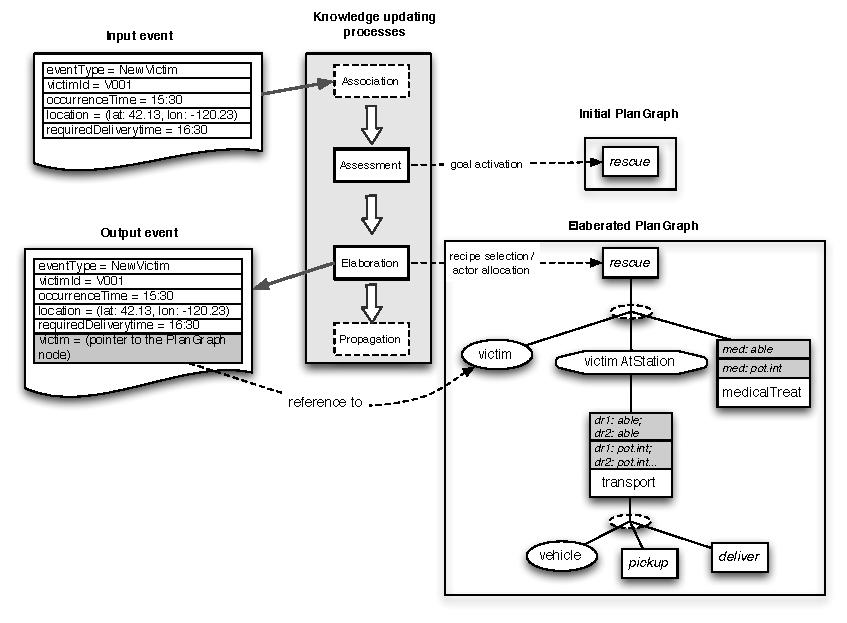
\includegraphics{update_example_event1.pdf} 
	\caption{The knowledge updating example (\emph{Event 1})}
	\label{fig:update_example_event1}
\end{figure}
% paragraph event_1_emph_newvictim (end)
\paragraph*{Event 2: \emph{`IntentionChange'}} % (fold)
\label{par:event_2_emph}
The second event is an internal event that is generated by the driver $dr_1$. After he interprets the first \emph{`NewVictim'} event, he decides that he has the intention to perform the \emph{`transport'} action to deliver this new victim to the medical station. As a result, he generates this \emph{`Intention'} event to update his intention on the \emph{`transport'} action from $pot.int$ to $int.to$. This \emph{`IntentionChange'} event has several key attributes, including the actor's id ($dr_1$), the action he intends to perform (\emph{`transport'}), and the intention type ($int.to$).

As the system receives this event, the system first attempts to associate it with any existing entities in the PlanGraph model. Because this is an intention event, the system traverses through the PlanGraph to search for any match between the action (\emph{`transport'}) mentioned in the event  and the action nodes in the PlanGraph. When the system is able to find such a match, the system uses the information in the event to update $dr_1$'s intention level on action \emph{`transport'}. Meanwhile, the corresponding attributes of the actor and the action in the event are updated with direct pointers to the nodes in the PlanGraph.

The knowledge updating process then proceeds to the following steps, but none of them leads to further changes in both the PlanGraph and the event itself. Figure \ref{fig:update_example_event2} shows the whole process performed on the second event.
\begin{figure}[htbp] %  figure placement: here, top, bottom, or page
	\centering
	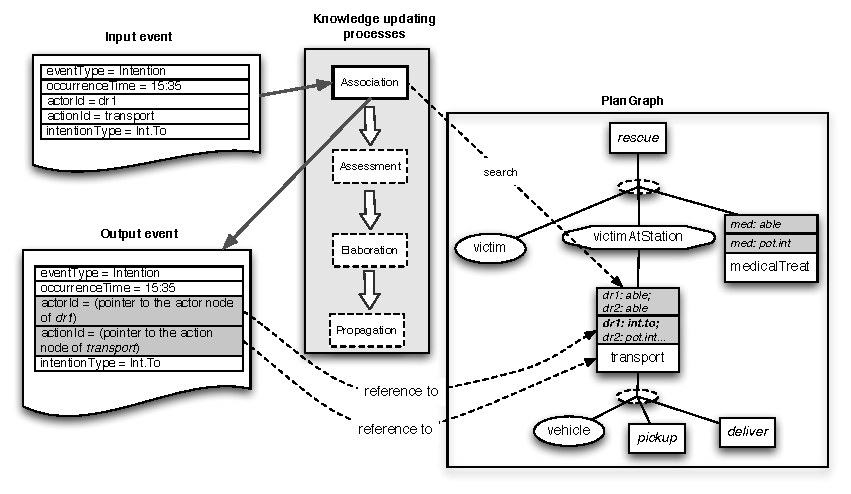
\includegraphics{update_example_event2.pdf} 
	\caption{The knowledge updating example (\emph{Event 2})}
	\label{fig:update_example_event2}
\end{figure}
% paragraph event_2_emph (end)

\paragraph*{Event 3: \emph{`FuelLevelLow'}} % (fold)
\label{par:event_3_}
The third event happens after driver $dr_1$ starts the action \emph{`transport'} and is on the way to pick up the victim. It is an external event indicating that the fuel level on driver $dr_1$'s vehicle is running extremely low. The event has an event type \emph{`FuelLevelLow'} and carries information about the driver, the vehicle, and the current fuel level. Figure \ref{fig:update_example_event3} shows the knowledge updating process performed on this event.

\begin{enumerate}
	\item When the event is first sent to the system, the system attempts to associate with any existing entities in the PlanGraph model. Because this is an external event indicating an attribute change on an entity, the system traverses through the PlanGraph to search for any match between the entity (\emph{`vehicle'}) mentioned in the event and the nodes in the PlanGraph. When the system is able to find such a match, the system uses the information in the event to update the value attached to parameter (\emph{`vehicle'}).
	\item Then the event is further processed in the assessment step, where the system checks whether the event can lead to changes towards the action performance. By checking the conditions attached with the parameter (\emph{`vehicle'}), the system finds that because of the low fuel level on the vehicle, the parameter becomes unavailable to perform the \emph{`transport'} action. As a result, a new state change event \emph{`ExecStatChange'} on the execution state of the parameter is derived, and added to the output event chain.
	\item As no new action nodes are added to the PlanGraph, the elaboration process is skipped.
	\item Because a state change event has been derived in the assessment step, the system attempts to predict future state changes in the field of work in the propagation step. A Bayesian network is constructed based on the current PlanGraph model and used to reason how likely the other entities in the PlanGraph will be impacted by the initial state change. After the Bayesian network-based reasoning, the system finds that the $dr_1$'s action to pick up the victim (\emph{`pickup'}) is likely to change its state from \emph{executing} to \emph{delaying}, and a new anticipatory event describing this state change on the execution state of the \emph{`pickup'} action is generated, and added to the output event chain.
\end{enumerate}

As we can see in Figure \ref{fig:update_example_event3}, after the knowledge updating process, the initial event is augmented into an event chain with three events: the original external event \emph{`FuelLevelLow'}, the execution state change event on the parameter \emph{`vehicle'} derived in the assessment step, and the anticipatory event predicting the execution state change event on the action \emph{`pickup'} in the propagation step. This example shows the idea that not only the knowledge representation of the field of work, i.e. PlanGraph model is updated because of the event, but also the PlanGraph model can enrich the original event with system generated knowledge that is used to support the human actor's awareness processes in following chapter.

\begin{figure}[htbp] %  figure placement: here, top, bottom, or page
	\centering
	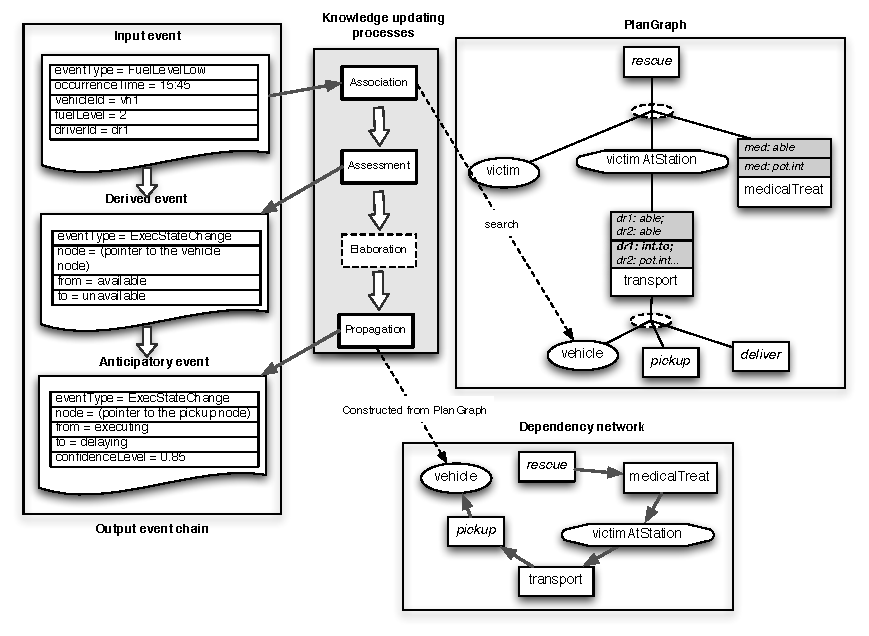
\includegraphics{update_example_event3.pdf} 
	\caption{The knowledge updating example (\emph{Event 3})}
	\label{fig:update_example_event3}
\end{figure}
% paragraph event_3_ (end)
% section an_example (end)
% chapter knowledge_updating (end)



 

